\documentclass[en]{../../../eplsummary}

\hypertitle{Design of Embedded and real-time systems}{8}{INGI}{2315}
{Charles-Henry Bertrand Van Ouytsel}
{Jean-Didier Legat}

\section{Give categories of real time task}
\begin{itemize}
    \item Hard : if result after the deadline can cause catastrophic consequences on the system
    \item Firm : if result after the deadline is useless for the system but can't cause any damage
    \item Soft : if result after the deadline has some utility although causing a performance degradation.
\end{itemize}
\section{What are the limits of current real time system ?}
\begin{itemize}
    \item \textbf{Multitasking :} Support for concurrent programming don't take time into account and introduce unbounded delay
    \item \textbf{Priority based scheduling :} Scheduling mechanism quite flexible but mapping with priority not always easy (limited number of priority level and arrival of a new task can lead to a remapping)
    \item \textbf{Ability to quickly respond to external interrupt :} If high priority to interrupt, application will always be interrupted even if it is more important than the driver to serve. Moreover, number of interrupt during an execution is non deterministic
    \item \textbf{Basic mechanism for process communication and synchronisation :} if no access protocol are used to enter in critical section, have to pay attention to some undesirable phenomena like priority inversion, chained blocking and deadlock which introduce unbounded delay.
    \item \textbf{Small kernel and fast context switch} : improve response time but doesn't give any guarantee  and implies limited functionality.
    \item \textbf{Support of a real-time clock as an internal time reference} : in many case, it's the only mechanism provided. No primitives for explicit timing constraints or activation of periodic task.
\end{itemize}
\section{Give the desirable features of a real-time system.}
\begin{itemize}
    \item [.]\textbf{Timeliness} : Result have to be correct in \textbf{value and time}. System needs to provide mechanisms for time management and handling tasks constraints/criticality. 
    \item [.] \textbf{Predictability} : System must be analyzable to predict the consequences of any scheduling decision. For example, knowing in advance if a time constraint will be violated to plan alternative actions.
    \item [.] \textbf{Efficiency} : Efficient management of the available resources (critical in most of the embedded system with severe constraints in term of space, memory, power, energy,..)
    \item [.] \textbf{Robustness} : System must be design to manage all anticipated load scenarios (be able to adapt to variables resources needs and high load variations).
    \item [.] \textbf{Fault tolerance} : Failure of software of hardware do not cause system to crash.
    \item [.] \textbf{Maintainability} : Architecture with modular structure to ensure easy possible modifications.
\end{itemize}
\section{What are the main sources of nondeterminism on the scheduling of the program}
\begin{itemize}
    \item [.] DMA
    \item [.] Cache
    \item [.] Interrupt
    \item [.] System Call
    \item [.] Semaphores
    \item [.] Memory management
    \item [.] Programming language
\end{itemize}
\section{Explain what is the DMA.}
DMA (direct memory access) is a technique used by peripheral device to transfer data between device and main memory. Its purpose is to relieve the CPU of the task of controlling I/O transfer. Since CPU andI/O device share the same bus, CPU has to be blocked when DMA device perform a data transfer. We have seen two methods for this transfer: 
\begin{itemize}
    \item [.] \textbf{Cycle stealing :} DMA device steal a CPU memory cycle in order to execute the data transfer. During DMA operation,  I/O transfer and CPU program execution run in parallel but if CPU requires a memory cycle at the same time, it's blocked and need to wait until end of DMA cycle. The main drawback of this method is thus than we have no way to predict how many time CPU will have to wait, so response time of a task can be precisely determined.
    \item [.] \textbf{Time slice method :} Each memory cycle is split into two adjacent time slots, one for CPU and one for DMA. This solution is more expensive but more predictable.
\end{itemize}
\section{Explain what is the cache.}
The cache is a fast memory that is inserted as a buffer between CPU and the RAM to speed up processes' execution. Once physical address of a memory location is determined, hardware checks whether the information is stored in the cache. If it is, data is read from the cache, otherwise it is taken from RAM and copied in cache along with a set of adjacent location (take advantage of program locality).\\
The cache introduce a degree of nondeterminism (data is not always present in the cache so data transfer is longer to copy data in cache, modification on the cache must be also done in memory,...). Last remark, in preemptive system, preemption destroy program locality and can reduce drastically efficacity of cache.
\section{Explain 3 different way to manage interrupt generated by I/O devices}
\begin{itemize}
    \item Disable all interrupts and handle peripherals device in application tasks. It allows programming flexibility and eliminates unbounded delay from interrupt drivers execution but cause low processor efficiency because of the busy wait of the task while accessing device registers.
    \item Disable all interrupts and handle peripherals device in dedicated kernel routines periodically activated by the timer. Again it eliminates unbounded delay from interrupt drivers execution and confines all I/O operation to one or more periodic kernel task which can encapsulate all hardware details and don't need to be known by application task. However busy wait of the kernel I/O handling routines are stil present, moreover the system overhead is higher due to communication between I/O kernel routines and applications task.
    \item Don't disable interrupt but their only purpose is through a simple driver task to activate a task that will take care of the device management. This task will be under the direct control of the OS and scheduled as other tasks. This method eliminates the busy wait during I/O operations and reduced the unbounded delay introduced by driver.
\end{itemize}
\section{What is a mutual exclusion ?}
The principle of mutual exclusion is that we must ensure each task has exclusive access on shared data structure at a given time to avoid data corruption. This can be done for example by mutex.

\section{Classification of scheduling algorithm}
\begin{itemize}
    \item Preemptive >< non preemptive (see next section)
    \item Static >< Dynamic : parameter of scheduling decision algorithm are fixed, assigned to task before execution >< parameter can change during execution
    \item Off-line >< Online : scheduling calculate before task activation >< scheduling decision taken at runtime.
    \item Optimal >< Heuristic : minimize some cost function >< use heuristic function, tend to optimal but doesn't guarantee it.
\end{itemize}
\section{Explain the concept of "guarantee-based algorithms"}
A guarantee-based algorithm is a class of scheduling algorithm which guarantee the feasibility of the schedule by assuming a worst case scenario. During runtime, a new task is accepted in the system if it is found schedulable, otherwise new task is rejected. Because, it's based of worst case scenario, it could reject unnecessarily task and leads to bad efficiency. However, it's really useful in hard real time system and allow to avoid problem like domino effect (arrival of a new task cause all previously guaranteed task to miss their deadlines.

\section{Explain the concept of "best-effort algorithms"}
A best-effort algorithm is a class of scheduling algorithm which tries to 'do its best' to meet deadlines, but there is no guarantee of finding a feasible schedule. Tasks can be abort during execution. These algorithm perform better than guarantee based algorithm in the average case because pessimistic assumption can unnecessarily cause task rejections where best effort algorithm abort task only in real overload condition.
\section{Give and explain the metrics for performance evaluation of a real-time OS}
Different metrics could be used to evaluate performance of a real-time OS:
\begin{itemize}
    \item Average response time :$t_r = \frac{1}{n} \sum^{n}_{i=1}(f_i - a_i)$
    \item Total completion time :$t_c = max(f_i) - min(a_i)$
    \item Weighted sum of completion time : $\sum^{n}_{i=1} w_i f_i$
    \item Maximum Lateness $L_{max} = max(f_i - d_i)$
    \item Maximum number of late task : $N_{late} = \sum^{n}_{i=1} miss(f_i)$ where $miss(f_i)$ equals 1 if task i miss its deadline. Good if soft deadlines.
\end{itemize}
$a_i$:  time task i is ready, $d_i$ = deadline of task i, $f_i$ time task i finish its execution
\section{Explain some scheduling anomalies:}
% Un dessin serait cool mais un peu la flemme :p 
Some scheduling anomalies are explained in the book, I won't explain them all but just give how task must be to see these anomalies : 
Suppose 9 task with following time of execution and decreasing priority: $J_1 (3)$,$J_2 (2)$,$J_3 (2)$,$J_4 (2)$,$J_5 (4)$,$J_6 (4)$,$J_7 (4)$,$J_8 (4)$,$J_9 (9)$. $J_1$ must be done before $J_9$ and $J_4$ before $J_{5,6,7,8}$. Initial schedule is done with 3 processors.\\
By drawing schedule, we can see that the following action increase total completion time:
\begin{itemize}
    \item Adding a processor
    \item Reduce each task by one unit of time.
    \item Remove constrain between $J_4$ and $J_{7,8}$
\end{itemize}
Other example can be found with resource constraint between processors, non-preemptive scheduling,...
\section{Explain the concept of foreground/background system}
A foreground/background system are system designed as follow : an application consist of an infinite loop that calls modules to perform the desired operations (background). ISR handle asynchronous events (foreground). Criticals operations have to be performed by ISR to ensure they are dealt with in a timely fashion. Also information for a background module made available by an ISR is not processed until the background routine gets it's turn to execute. So the task level response depends on how long the main loop takes to execute.
\section{Explain the concept of "priority inversion" and "priority inheritance"}
Priority inversion is a problem which occurs in real time system when a high-priority task T1 is blocked by a low-priority task T2 for an unbounded interval of time for example because of a resource protected by a mutex. It can be worst if another task T3 with higher priority than T2 but lower priority than T1 start to execute ( T1 will thus execute after T3 and the release of the mutex by T2).
\\
A solution to this problem is priority inheritance : we modify priority of the task based of the current use of the resource and control resource assignment at the entrance of each critical section.
\section{Explain the concept of "non-preemptive and preemptive kernels"}
Non-preemptive Kernels requires that \textbf{each task does something to explicitly give up control of the CPU}. To maintain illusion of concurrency, this process must be done frequently. Interrupt preempt a task, after ISR return to  the interrupted task. Its advantages are : allow use of non-reentrant function, interrupt latency lower, less use of semaphore, better in task level responsiveness than foreground/background system. Its main drawback is its bad an non deterministic responsiveness with respect to higher task.
\\
Preemptive kernel \textbf{always execute the highest priority task} which is ready to run. So current task may be interrupt if a higher task is ready to run. An interrupt preempts a task. Upon completion of the ISR, kernel resume to the highest priority task ready to run. This leads to a task level response optimum and deterministic. However, it's important to use protection for shared data and to not use non-reentrant function.




\section{What are the Interrupt Latency, Response, and Recovery ?}
Interrupt latency : maximum amount of time interrupts are disabled + Time to start executing the first instruction of the ISR.
\\
Interrupt response : time between reception of an interrupt and start of the user code that handles the interrupt. It takes into account all overhead involved in handling the interrupt (for example Time to save the CPU's context, ISR entry function for preemptive kernel..) and the interrupt latency.
\\
Interrupt recovery: time required by the CPU to return to an interrupted code or to an higher priority task (preemptive kernel). Generally it's calculated as : Time to restore CPU context + time to return to the interrupted instruction (+ time to determine if a higher priority task is available).

\section{Explain the concept of Deadlock}
A deadlock is a situation in which two tasks are each unknowingly waiting for resources held by the other. For example T1 has exclusive access on R1 and wait for R2 and T2 has exclusive access on R2 and wait for R1. To avoid this, each task must : try to acquire all resource before processing, acquire resource in the same order and release them in the reverse order.

\newpage

\section{Solutions of the book Hard Real Time Computing Systems}
\subsection*{Chapter 1}
\begin{center}
    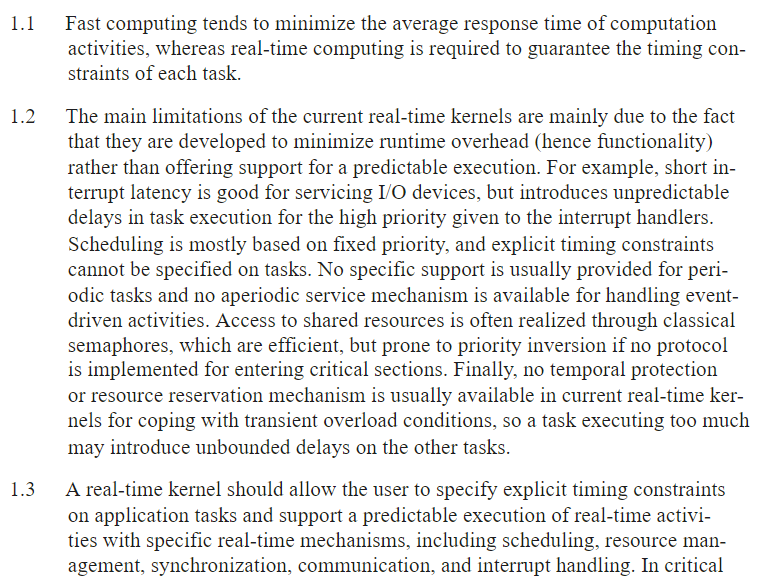
\includegraphics[scale=0.8]{hard1}\\
    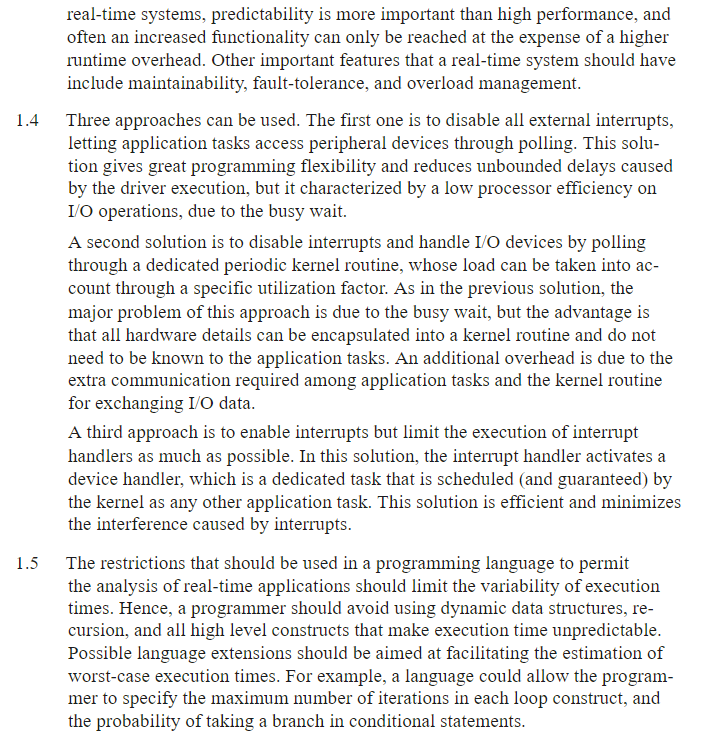
\includegraphics[scale=0.8]{hard11}
\end{center}

\subsection*{Chapter 2}
\begin{center}
    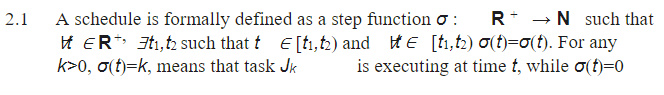
\includegraphics[scale=0.8]{hard2}\\
    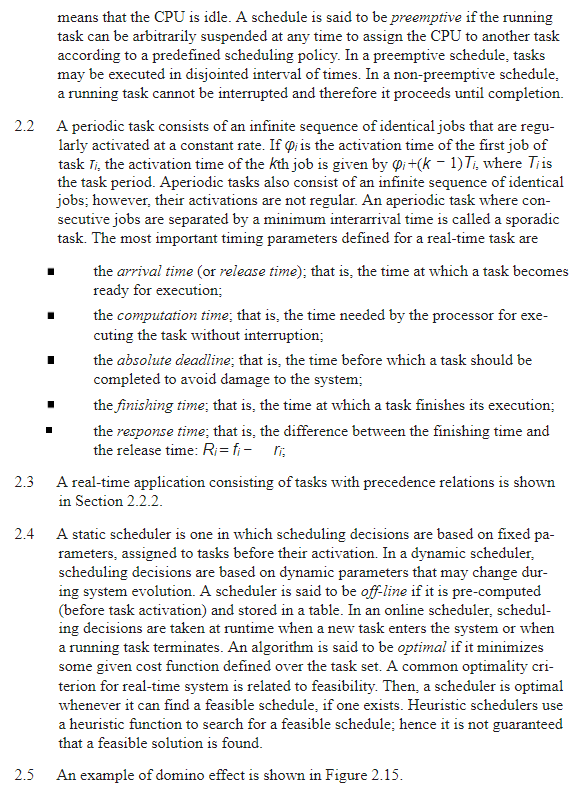
\includegraphics[scale=1]{hard22}
\end{center}

\end{document}
